\documentclass[11pt]{article}\usepackage[]{graphicx}\usepackage[]{color}
%% maxwidth is the original width if it is less than linewidth
%% otherwise use linewidth (to make sure the graphics do not exceed the margin)
\makeatletter
\def\maxwidth{ %
  \ifdim\Gin@nat@width>\linewidth
    \linewidth
  \else
    \Gin@nat@width
  \fi
}
\makeatother

\definecolor{fgcolor}{rgb}{0.345, 0.345, 0.345}
\newcommand{\hlnum}[1]{\textcolor[rgb]{0.686,0.059,0.569}{#1}}%
\newcommand{\hlstr}[1]{\textcolor[rgb]{0.192,0.494,0.8}{#1}}%
\newcommand{\hlcom}[1]{\textcolor[rgb]{0.678,0.584,0.686}{\textit{#1}}}%
\newcommand{\hlopt}[1]{\textcolor[rgb]{0,0,0}{#1}}%
\newcommand{\hlstd}[1]{\textcolor[rgb]{0.345,0.345,0.345}{#1}}%
\newcommand{\hlkwa}[1]{\textcolor[rgb]{0.161,0.373,0.58}{\textbf{#1}}}%
\newcommand{\hlkwb}[1]{\textcolor[rgb]{0.69,0.353,0.396}{#1}}%
\newcommand{\hlkwc}[1]{\textcolor[rgb]{0.333,0.667,0.333}{#1}}%
\newcommand{\hlkwd}[1]{\textcolor[rgb]{0.737,0.353,0.396}{\textbf{#1}}}%
\let\hlipl\hlkwb

\usepackage{framed}
\makeatletter
\newenvironment{kframe}{%
 \def\at@end@of@kframe{}%
 \ifinner\ifhmode%
  \def\at@end@of@kframe{\end{minipage}}%
  \begin{minipage}{\columnwidth}%
 \fi\fi%
 \def\FrameCommand##1{\hskip\@totalleftmargin \hskip-\fboxsep
 \colorbox{shadecolor}{##1}\hskip-\fboxsep
     % There is no \\@totalrightmargin, so:
     \hskip-\linewidth \hskip-\@totalleftmargin \hskip\columnwidth}%
 \MakeFramed {\advance\hsize-\width
   \@totalleftmargin\z@ \linewidth\hsize
   \@setminipage}}%
 {\par\unskip\endMakeFramed%
 \at@end@of@kframe}
\makeatother

\definecolor{shadecolor}{rgb}{.97, .97, .97}
\definecolor{messagecolor}{rgb}{0, 0, 0}
\definecolor{warningcolor}{rgb}{1, 0, 1}
\definecolor{errorcolor}{rgb}{1, 0, 0}
\newenvironment{knitrout}{}{} % an empty environment to be redefined in TeX

\usepackage{alltt}
%\usepackage[showframe]{geometry}
\usepackage[table]{xcolor}
\usepackage{caption}
\usepackage{lscape,verbatim,mathrsfs}
\usepackage{graphics,amsmath,pstricks}
\usepackage{amssymb,enumerate}
\usepackage{amsbsy,amsmath,amsthm,amsfonts, amssymb}
\usepackage{graphicx, rotate, array}
\usepackage{geometry,multirow}
\usepackage{color,soul}
\usepackage{float}
%\usepackage{hyperref}
\usepackage[authoryear,round]{natbib}
%\renewcommand{\baselinestretch}{1.9}
\usepackage{tcolorbox}
\renewcommand{\familydefault}{cmss}
\textwidth=6.65in \textheight=9.7in
\parskip=.025in
\parindent=0in
\oddsidemargin=-0.1in \evensidemargin=-.1in \headheight=-.6in
\footskip=0.5in \DeclareMathOperator*{\argmax}{argmax}
\DeclareMathOperator*{\argmin}{argmin}
\IfFileExists{upquote.sty}{\usepackage{upquote}}{}
\begin{document}









bin







\begin{knitrout}
\definecolor{shadecolor}{rgb}{0.969, 0.969, 0.969}\color{fgcolor}
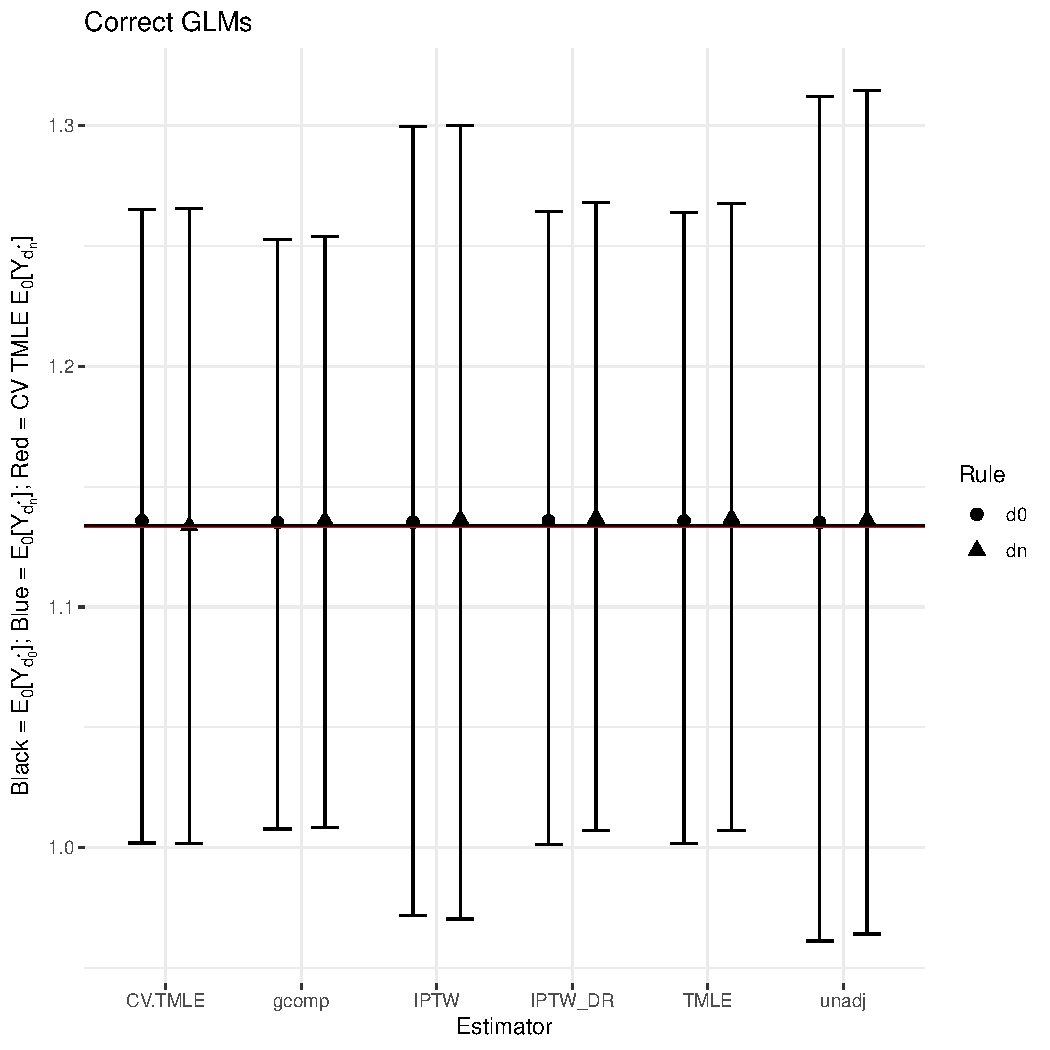
\includegraphics[width=\maxwidth]{figure/unnamed-chunk-1-1} 

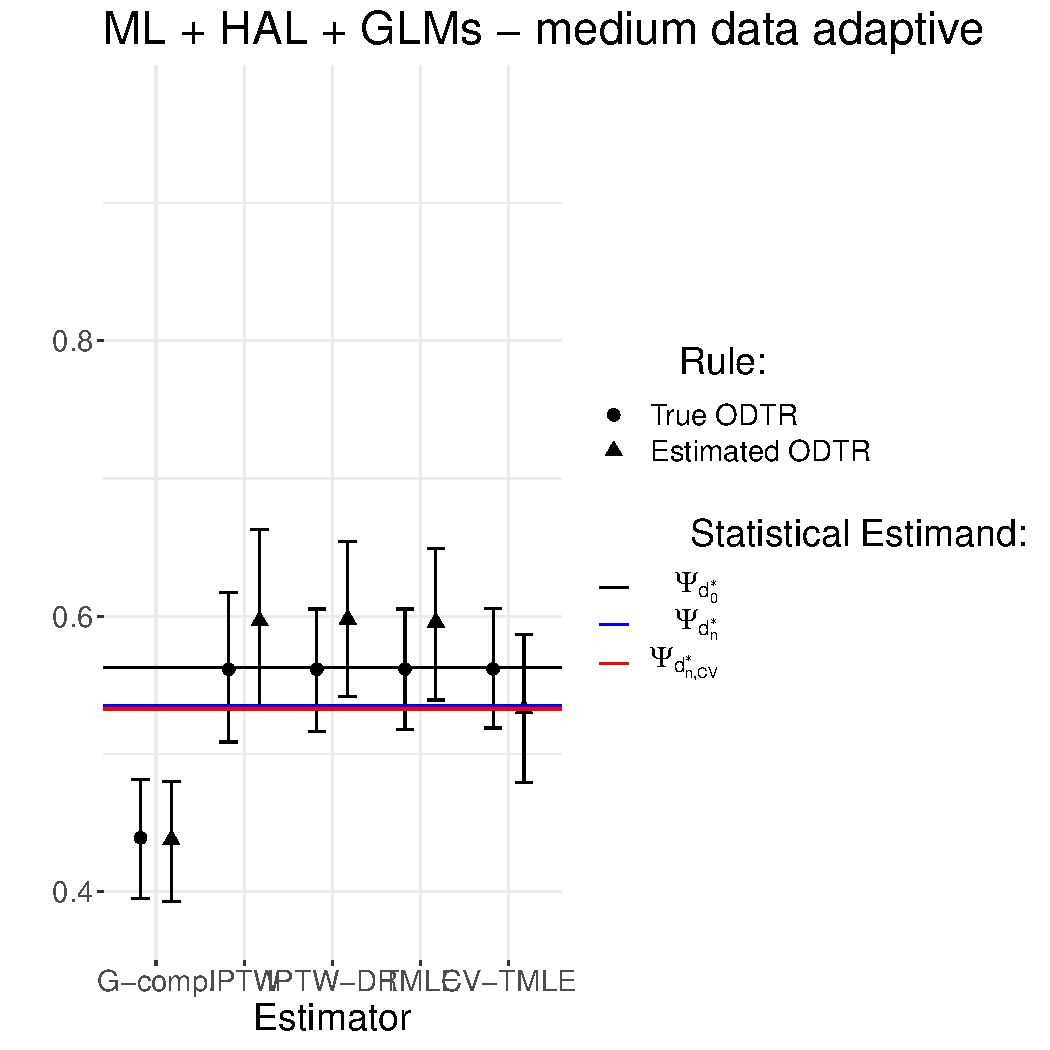
\includegraphics[width=\maxwidth]{figure/unnamed-chunk-1-2} 

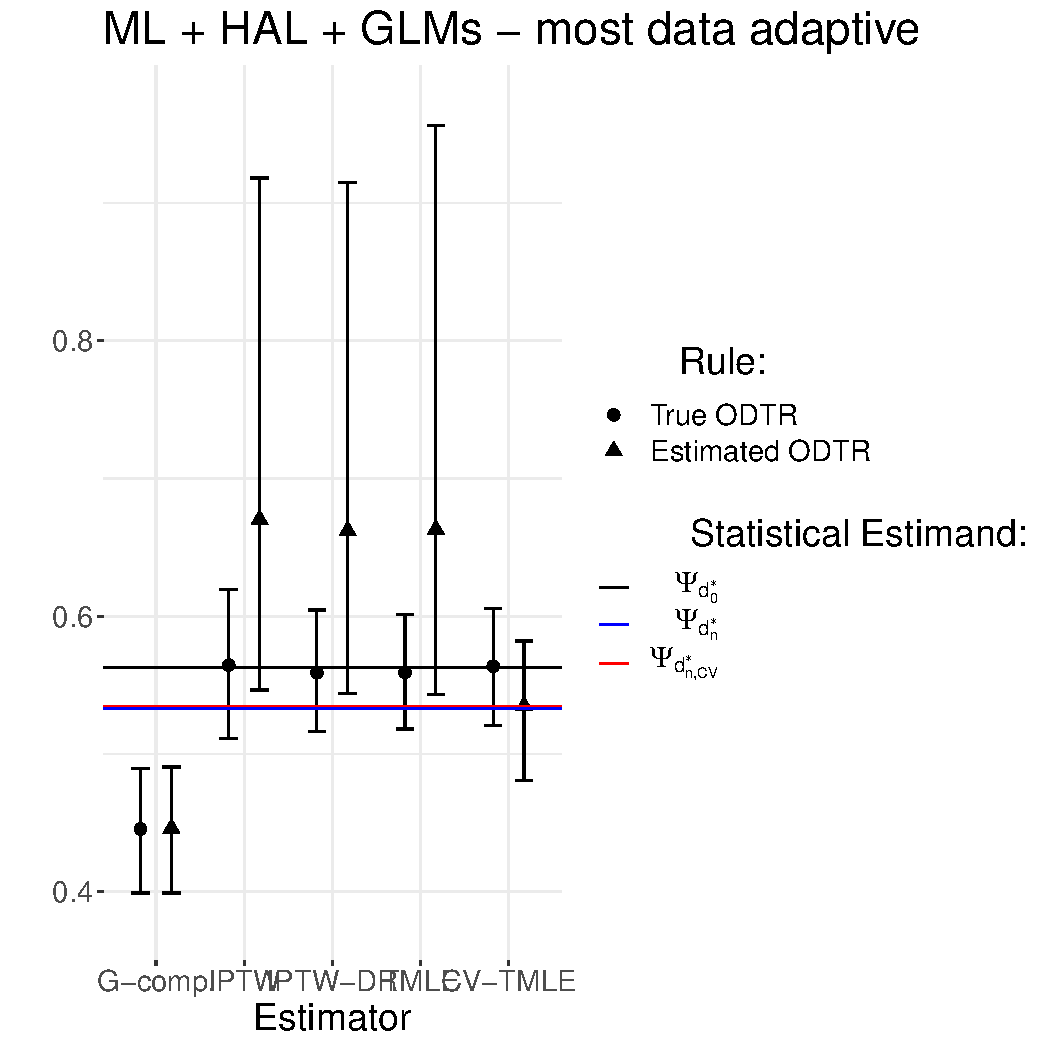
\includegraphics[width=\maxwidth]{figure/unnamed-chunk-1-3} 

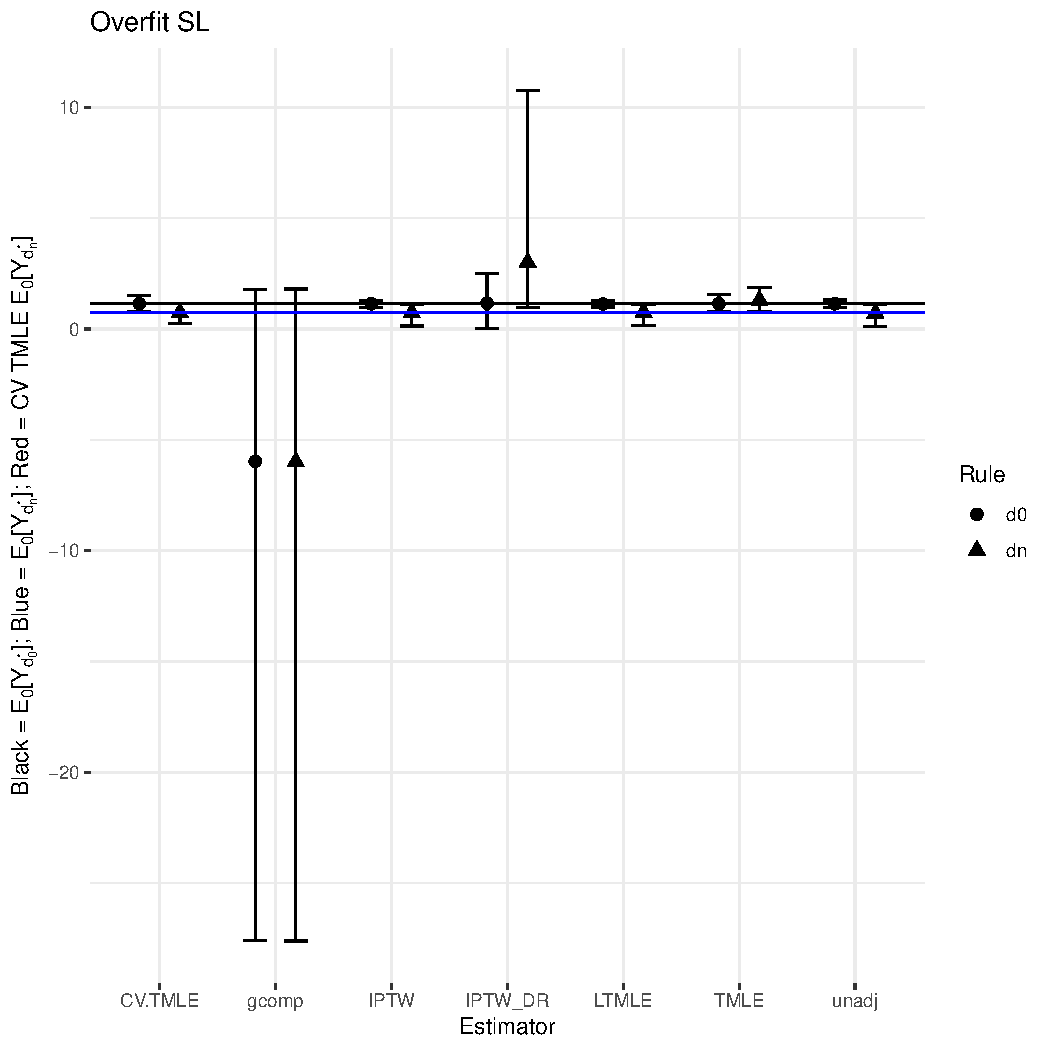
\includegraphics[width=\maxwidth]{figure/unnamed-chunk-1-4} 

\end{knitrout}

\begin{knitrout}
\definecolor{shadecolor}{rgb}{0.969, 0.969, 0.969}\color{fgcolor}\begin{kframe}
\begin{alltt}
\hlcom{# Incorrect GLM}
\hlkwd{make_table_EYdopt}\hlstd{(}\hlkwc{EYdopt} \hlstd{= EYdopt_step2_bin,} \hlkwc{truevalues} \hlstd{= DGP_AL_bin_true_values)}
\end{alltt}
\begin{verbatim}
##                     Bias Variance    MSE Coverage
## unadj            -0.0601    6e-04 0.0042    0.519
## gcomp            -0.0615    4e-04 0.0042        -
## IPTW             -0.0613    8e-04 0.0045    0.387
## IPTW_DR            -0.06    6e-04 0.0042    0.243
## TMLE               -0.06    6e-04 0.0042    0.243
## LTMLE                  -        -      -        -
## CV.TMLE          -0.0798    8e-04 0.0071    0.091
## unadj_dopt0       -5e-04    6e-04  6e-04     0.99
## gcomp_dopt0      -0.0922    3e-04 0.0088        -
## IPTW_dopt0       -0.0011    9e-04  9e-04     0.94
## IPTW_DR_dopt0     -8e-04    5e-04  5e-04    0.925
## TMLE_dopt0        -7e-04    5e-04  5e-04    0.933
## LTMLE_dopt0            -        -      -        -
## CV.TMLE_dopt0     -3e-04    5e-04  5e-04    0.933
## unadj_sampspec     0.017    6e-04  7e-04    0.987
## gcomp_sampspec    0.0157    4e-04  7e-04        -
## IPTW_sampspec     0.0158    8e-04  8e-04    0.947
## IPTW_DR_sampspec  0.0171    6e-04  7e-04    0.916
## LTMLE_sampspec         -        -      -        -
## TMLE_sampspec     0.0172    6e-04  7e-04    0.914
## CV.TMLE_sampspec   1e-04    8e-04  5e-04    0.939
\end{verbatim}
\begin{alltt}
\hlcom{# Non-overfit SL}
\hlkwd{make_table_EYdopt}\hlstd{(}\hlkwc{EYdopt} \hlstd{= EYdopt_step3_bin,} \hlkwc{truevalues} \hlstd{= DGP_AL_bin_true_values)}
\end{alltt}
\begin{verbatim}
##                     Bias Variance    MSE Coverage
## unadj            -0.0612    7e-04 0.0044    0.487
## gcomp            -0.0931    3e-04 0.0090        -
## IPTW             -0.0608    8e-04 0.0045    0.388
## IPTW_DR          -0.0606    7e-04 0.0043    0.266
## TMLE             -0.0606    7e-04 0.0043    0.266
## CV.TMLE          -0.0826    8e-04 0.0077    0.091
## unadj_dopt0      -0.0010    5e-04 0.0005    0.996
## gcomp_dopt0      -0.0983    3e-04 0.0099        -
## IPTW_dopt0       -0.0007    9e-04 0.0009    0.945
## IPTW_DR_dopt0    -0.0011    5e-04 0.0005    0.952
## TMLE_dopt0       -0.0010    5e-04 0.0005     0.95
## CV.TMLE_dopt0    -0.0009    5e-04 0.0005    0.947
## LTMLE            -0.0621    7e-04 0.0045    0.236
## LTMLE_dopt0      -0.0013    5e-04 0.0005    0.953
## unadj_sampspec    0.0180    7e-04 0.0007    0.987
## gcomp_sampspec   -0.0138    3e-04 0.0008        -
## IPTW_sampspec     0.0185    8e-04 0.0009    0.941
## IPTW_DR_sampspec  0.0187    7e-04 0.0007    0.912
## LTMLE_sampspec    0.0172    7e-04 0.0007    0.922
## TMLE_sampspec     0.0187    7e-04 0.0007    0.912
## CV.TMLE_sampspec -0.0003    8e-04 0.0006    0.933
\end{verbatim}
\begin{alltt}
\hlcom{# Overfit SL}
\hlkwd{make_table_EYdopt}\hlstd{(}\hlkwc{EYdopt} \hlstd{= EYdopt_step4_bin,} \hlkwc{truevalues} \hlstd{= DGP_AL_bin_true_values)}
\end{alltt}
\begin{verbatim}
##                     Bias Variance    MSE Coverage
## unadj             0.0156    6e-04 0.0009    0.968
## gcomp            -0.1416    7e-04 0.0208        -
## IPTW              0.0218    9e-04 0.0014    0.875
## IPTW_DR           0.0206    7e-04 0.0011    0.829
## TMLE              0.0185    7e-04 0.0010    0.831
## CV.TMLE          -0.0334    8e-04 0.0019    0.666
## unadj_dopt0      -0.0007    5e-04 0.0005    0.994
## gcomp_dopt0      -0.1397    6e-04 0.0201        -
## IPTW_dopt0       -0.0009    8e-04 0.0008    0.951
## IPTW_DR_dopt0    -0.0015    5e-04 0.0005    0.952
## TMLE_dopt0       -0.0014    5e-04 0.0005     0.95
## CV.TMLE_dopt0    -0.0007    5e-04 0.0005    0.953
## LTMLE             0.0046    6e-04 0.0006    0.917
## LTMLE_dopt0      -0.0021    4e-04 0.0004    0.952
## unadj_sampspec    0.0429    6e-04 0.0024      0.8
## gcomp_sampspec   -0.1143    7e-04 0.0140        -
## IPTW_sampspec     0.0492    9e-04 0.0032    0.594
## IPTW_DR_sampspec  0.0480    7e-04 0.0029    0.449
## LTMLE_sampspec    0.0320    6e-04 0.0015    0.664
## TMLE_sampspec     0.0458    7e-04 0.0027    0.474
## CV.TMLE_sampspec -0.0008    8e-04 0.0005    0.929
\end{verbatim}
\begin{alltt}
\hlcom{# Very overfit SL (with RF)}
\hlkwd{make_table_EYdopt}\hlstd{(}\hlkwc{EYdopt} \hlstd{= EYdopt_step5_bin,} \hlkwc{truevalues} \hlstd{= DGP_AL_bin_true_values)}
\end{alltt}
\begin{verbatim}
##                     Bias Variance    MSE Coverage
## unadj             0.1404   0.0143 0.0340    0.353
## gcomp            -0.1140   0.0008 0.0138        -
## IPTW              0.1493   0.0136 0.0359    0.297
## IPTW_DR           0.1115   0.0104 0.0228    0.329
## TMLE              0.1194   0.0131 0.0273    0.323
## CV.TMLE          -0.0326   0.0007 0.0018    0.655
## unadj_dopt0      -0.0010   0.0005 0.0005    0.997
## gcomp_dopt0      -0.1175   0.0007 0.0145        -
## IPTW_dopt0       -0.0009   0.0007 0.0007    0.958
## IPTW_DR_dopt0    -0.0129   0.0005 0.0006    0.883
## TMLE_dopt0       -0.0116   0.0005 0.0006    0.882
## CV.TMLE_dopt0    -0.0011   0.0005 0.0005    0.944
## LTMLE             0.0943   0.0104 0.0192    0.376
## LTMLE_dopt0      -0.0106   0.0004 0.0005    0.891
## unadj_sampspec    0.1733   0.0143 0.0471    0.238
## gcomp_sampspec   -0.0812   0.0008 0.0077        -
## IPTW_sampspec     0.1821   0.0136 0.0493    0.166
## IPTW_DR_sampspec  0.1443   0.0104 0.0334    0.184
## LTMLE_sampspec    0.1272   0.0104 0.0290     0.24
## TMLE_sampspec     0.1522   0.0131 0.0389    0.175
## CV.TMLE_sampspec -0.0016   0.0007 0.0005    0.952
\end{verbatim}
\end{kframe}
\end{knitrout}




\end{document}
